%--------------------------------------------------------------------
%	(c) SPP 2014
%   This is a pragmatic LaTeX conversion of the MS Word document
%   stating the required format for the submission of articles 
%   for consideration in the SPP Physics Congress.  This template
%   includes the rules on formatting your article and thus before
%   editing it typeset it first to produce a postscript/pdf file
%   that you can read.  Use the latex, dvips, and ps2pdf commands 
%   to typeset the template directly into a pdf file.  Make sure 
%   to place the included figure in the same directory as the 
%   template.  This template uses standard LaTeX packages latexsym,
%   graphicx, geometry, fancyhdr, caption, and cite.
%
%   Note, in particular, the format used to typeset figures and
%   tables.  Since SPP requires figure/table captions to be
%   within an inch of the figure/table, you must define manually
%   the width of the caption at the beginning of the figure/table
%   environment.
%-------------------------------------------------------------------
\documentclass[twoside]{article}

\usepackage{latexsym}      % needed math symbols
\usepackage{graphicx}      % for importing eps figures
\usepackage{caption}
\usepackage{subcaption}
\usepackage{multirow}
% paper and margin formats as set by SPP
\usepackage[margin=1.0in,papersize={21.0cm,29.7cm}]{geometry}

\parindent 0.5cm    % paragraphs indent
\newcommand{\changefont}{%
    \fontsize{9}{10}\selectfont
}

% for the footer
\usepackage{fancyhdr}
\fancyhf{}
\renewcommand{\headrulewidth}{0pt}
\renewcommand{\footrulewidth}{0.5pt}
\tiny
\fancyfoot[c]{\changefont
Physics 191\\
National Institute of Physics, Diliman, Quezon City\\
15 September 2016 \\
\thepage}

\pagestyle{fancy}


% for section formatting style
\makeatletter
\renewcommand\section{\@startsection
   {section}{1}{0pt}%
   {-\baselineskip}%
   {0.1\baselineskip}%
   {\normalfont\large\bfseries}}%
\makeatother
\renewcommand\thesection{\arabic{section}.}

% for the figure captions
\usepackage{caption}
\captionsetup[table]{position=top,aboveskip=5pt,font={rm,small}}
\captionsetup[figure]{font={rm,small}}

% for citations formatting style
\usepackage[compress,nospace]{cite}

\begin{document}

%--------------------------------------------------------------------------
%  fill in the paper's title, author(s), and corresponding institutions
%--------------------------------------------------------------------------
\begin{center}
{\Large\textbf{Properties of white light and of the primary colors of light}}\\
\vspace{0.05in}
\textbf{Joshua Carlo Casapao, David Bryan Lao, and Jan Carlo Lima$^{\ast}$}\\
\textit{University of the Philippines, National Institute of Physics, Diliman, Quezon City}\\
\textrm{$^{\ast}$Corresponding author: lima.jcarlo@gmail.com}\\

\vspace{0.15in}


%--------------------------------------------------------------------------
%                    Abstract
%--------------------------------------------------------------------------
\parbox{4.5in}{{\large \textbf{Abstract}}\\
\noindent{White light, when dispersed, exhibits a continuous spectrum. The bands of the spectrum correspond to certain colors.  The light from each of these bands have interesting visual properties.  They can be added, subtracted or even used to produce colored shadows.  The experiment then investigates these different properties, using colored spotlights and flashlights as sources, along with the effects of filters on colored lights and pictures.  The dispersion of light was also exhibited using a rhombus prism.  It was found out that the separation happens at around $36^{\circ}$ from the normal.  Also, we find that red is refracted at the least angle while violet is refracted the most.  Thus, Snell's law is proven to have governed the experiment. }\\

\noindent{Keywords: dispersion, color addition, color subtraction}}\\
\end{center}

%---------------------------------------------------------------------------
%               Section 1 : Introduction
%---------------------------------------------------------------------------
\section{Introduction}
\label{sec:intro}

Much of the perceived daylight spectrum here on Earth is white light, which Newton first recognized as a mixture of all the colors of the visible spectrum that are more or less non-dominating in intensity \cite{Hecht}. His observation came about when a beam of white light was projected on a glass prism which separated the white light into different visible wavelengths, hence the different perceived colors, with each wavelength refracted at different angles \cite{Bauer}.  The entirety of the refracted wavelengths was again projected to another prism which let Newton retrieve back the white light. Today, the refraction at the boundary between two optical media resulting to different wavelengths is called chromatic dispersion \cite{Bauer}. In this experiment, the dispersion of white light using one prism was observed by noting Snell’s law of refraction:

\begin{equation}
n_i \sin{\theta_i} = n_r (\lambda)\sin{\theta_r (\lambda)}
\label{eqn:Snell}
\end{equation}

\noindent Here, $n$ and $\theta$ indicate the refractive index and angular displacement from the surface normal, respectively. Also, $i$ indicates the incident white light beam from air, and $r$ the refracted beam of wavelength $\lambda$ that is qualitatively described by the perceived color. It is clear from Equation (1) that the refractive index $n_r$ changes with the color. 

To produce white light, a uniform intensity distribution across all wavelengths in the visible spectrum, like mentioned before, is not necessary. Any three visible beams, all widely separated and all having the same intensity, which produce white light when combined are called primary colors \cite{Hecht}. In this paper, the primary colors used were red, green, and blue. Any combination of two primary colors of the same intensity is referred to as a secondary color. Varying the intensity of the primary colors was also done, which raises the notion of color saturation for the resulting light combination that is not necessarily white.

For an incident light (a superposition of different wavelengths) hitting a certain material, a portion of this light will be strongly or preferentially absorbed, while the remaining parts will be either reflected back or be transmitted through the material. If some fraction of the light is absorbed, it means that this fraction matches any of the visible resonant frequencies of the material, hence vibrations occurring in the molecular level \cite{Hecht}. Since the remaining fraction, hereafter referred to as the complementary light of the absorbed part, contributes none to the vibrations, it is reflected back (or transmitted) as the perceived color. In this experiment, this process of subtractive coloration was observed by means of light filters (based primarily on absorption) and colored shadows (based on the complementary light) with the given primary colors.


%-------------------------------------------------------------------------
%                              Section 2 : Methodology
%-------------------------------------------------------------------------
\section{Methodology}
\label{sec:methods}

	For the first part of the experiment, a picture of a parrot was used to investigate the effects of filters (red, blue and green).  The filters were placed in the lens of the camera, and the parrot picture was photographed.  The results were recorded.

For the second part of the experiment, color separation was studied using a flashlight, a cylindrical lens, a rhombus prism, a rotating stage and a white paper screen.  The rhombus prism is made of acrylic which has an index of refraction of $1.497$ for light of wavelength $486$ nm, $1.491$ for wavelength $589$ nm, and $1.489$ for wavelength $651$ nm. The flashlight was placed a short distance from the rotating stage, on top of which the rhombus prism was positioned.  Between the flashlight and the stage, a cylindrical lens was included to focus the rays, allowing a single, thin ray to pass through.  Beyond the rotating stage, a white paper screen was placed so that the emergent ray can be observed. After measurements were done, the prism was rotated until the optimal color separation was obtained.  The results were then documented.

For the third part, color addition was investigated using three flashlights, filters (red, blue and greed), a convex lens and a white paper screen.  The three flashlights were held relatively far from the screen.  Each flashlight was covered with a filter.  The rays were then adjusted so that they all entered the convex lens and were projected on the black screen.  The flashlights were then moved until the three projected images overlap with each other in a manner resembling a Venn diagram of three sets.  The results were documented.
	
    For the fourth part, color subtraction was studied using the same spotlights, the color wheel, and the filters mentioned above.  The effects of the different filters on the different colors and color combinations made by the spotlights were investigated, the process being similar to what was done to the parrot picture.  The results were documented.
	
    For the fifth part, color addition was investigated using the same set of spotlights.  This was done, basically, by mixing two colors at a time for the different combinations and finally mixing all of them.  The results were then noted.
	
    For the sixth part, complementary colors were studied via the same spotlights.  This was achieved by turning on two spotlights at a time then turning the remaining one after and documenting the result.  The process was then repeated for all possible combinations.
	
    For the seventh part, colored shadows were investigated.  The study was done using the same spotlights, some hands to produce the shadow and a screw on the wall to do the same.  The phenomenon was then studied by first turning on one light, and then turning on two lights and then turning on three, documenting the results every time.  
	
    For the last part of the experiment, advanced color addition was studied.  A list of colors was presented (orange, pink, purple and brown) to be formed using the three spotlights.  The various results were then properly documented.      



%-------------------------------------------------------------------------
%                              Section 3 : RnD
%-------------------------------------------------------------------------

\section{Results and Discussion}
\label{sec:RnD}

The colors of the parrot image are shown in Figure 1. Since only one primary color of light was allowed through the respective filters, the other colors looked dimmer than they are under unfiltered light. This can be seen in Figure 2.

The separated colors of light are shown in Figure 4. The separation happens at around $36^{\circ}$ from the normal. From bottom to top, the colors seen are red, orange, yellow, green, blue, and violet. Violet is refracted at the largest angle and red at the lowest angle, as can be predicted through Snell's law. This is because of the given index of refraction depending on the wavelength of the incident light.

The three flash lights resembled Venn diagrams with the intersections being the added lights and the center being white. This can be seen in Figure 5. Blue and green mix to reveal cyan, blue and red show magenta, and red and green mix to form yellow. When two colors are added, the resulting wavelength of the light is the averages of the incident wavelengths of light. This can be observed in a spectrum of colors: in the middle of red and green is yellow, with blue and red is magenta, and with blue and green is cyan. When one light is more intense than another, the observer sees this light as having more of white than the original color. Thus the difference in addition shall be seen.

The resulting colors of the wheel after being filtered can be seen in Figure 3. The primary colors in spotlights were filtered and those images can be seen in Figure 6. As with the parrot, the colors of the circles appear as stated in Table 1:

\captionsetup[table]{width=4in}
\begin{table}[h!]
\centering
\caption{Appearance of the colored circles on the color wheel viewed through the colored filters.}
\begin{tabular}{ |c|c|c|c| } 
\hline
Color on monitor & Color of filter & Color of transmitted light \\
\hline
\multirow{3}{4em}{Red} & red & red \\ 
					   & green & gray \\ 
					   & blue & black \\ 
\hline
\multirow{3}{4em}{Green} & red & black \\ 
					     & green & green \\ 
					     & blue & gray \\ 
\hline
\multirow{3}{4em}{Blue} & red & gray \\ 
					    & green & black \\ 
					    & blue & blue \\ 
\hline
\multirow{3}{4em}{Yellow} & red & red \\ 
					      & green & green \\ 
					      & blue & gray \\ 
\hline
\multirow{3}{4em}{Cyan} & red & gray \\ 
					    & green & green \\ 
					    & blue & blue \\ 
\hline
\multirow{3}{4em}{Magenta} & red & red \\ 
					       & green & gray \\ 
					       & blue & blue \\ 
\hline
\end{tabular}
\label{tab:mytab}
\end{table}

The result of the filtering of the color wheel shows how the secondary colors, cyan, yellow and magenta, are composed of two primary colors. When the the yellow circle is seen through the green filter, it looks green and through the red filter, it looks red. It becomes gray when it is viewed through the blue filter, blue not being part of it at all.

The images for the parts of the experiment which used spotlights can be found in Appendix C. Adding two primary colors resulted in a secondary color, adding blue and green form cyan, red and blue form magenta, and red and green form yellow. This result, seen in Figure 7, is consistent with color addition using the light ray box.

It has been confirmed that the complementary colors of blue, red and green light are yellow, cyan, and magenta, respectively. This can be seen in Figure 8.

The colored shadows part of the experiment uses the above result for its concept. Seen in Figure 9, from left to right, the screw was shone with blue light. The resulting shadow was black as the screw blocked all light source. Green was added and the shadows became colored. The shadow of the blue light is green while the shadow of the green is blue. This is because when cyan is shone on the screw, if it blocks only the blue light the color of the shadow is the portion of the light that is left. When the two colors are from the same point, the shadow is black since the screw blocks all light colors. Red is added and the secondary colors appear. This is because of the concept of complementary colors. The shadow of the blue light is yellow since all that is left is red and green, and so on for the other two. Again, if the three spotlights were from the same point, the shadow will be black since all light is blocked (or an absence of white light).

To create the colors required, the spotlights were arranged in order to form the secondary colors. One light was made to be dimmer than the other light and together they formed the wanted colors. These colors can be seen in Figure 10.

\captionsetup[table]{width=4in}
\begin{table}[h!]
\centering
\caption{Guide on how to form the colors needed for the experiment.}
\begin{tabular}{||c|c|c||}
\hline
Need & Dimmer Color & Brighter Color \\ \hline \hline
Purple & Red & Blue \\ \hline
Pink & Blue & Red \\ \hline
Orange & Green & Red \\ \hline
Brown & Red & Green \\ \hline
\end{tabular}
\label{tab:mytab}
\end{table}

It was observed that for the camera, the spotlight should be dimmed a bit since when the light is on full-blast, the camera detects it as having more white, or saturated, and would cause the mixing and the filtering to be off in terms of color.

%-------------------------------------------------------------------------
%                              Section 4 : Conclusion
%-------------------------------------------------------------------------

\section{Conclusion and Recommendation}
\label{sec:conclusion}

Th objectives of the experiment were met as the processes of additive coloration, subtractive coloration, and color separation was observed by means of spotlights, light filters (based primarily on absorption) and colored shadows (based on the complementary light) with the given primary colors, and prisms, respectively.

Results obtained in the experiment proved to be consistent with the Snell's law (separation) and the recognized text. White is indeed made of various wavelengths of light, thus many colors can be perceived once the light is separated.

The perception of the human eye is thus because of the white light from the sun and from the artificial lights that have been made throughout the years. If the sun were red and thus our man-made lights red as well, then the human eye will perceive different colors. Such was found that if red light were shone on a color other than red, that color would be perceived as gray or black depending on the saturation of the said color.

%-------------------------------------------------------------------------
%                              References
%-------------------------------------------------------------------------

\newpage

\begin{thebibliography}{100}
\bibitem{Hecht}
E. Hecht. Optics, 4th Ed. Pearson Education, Inc. California, USA (2002).
\bibitem{Bauer}
W. Bauer, G. Westfall. University Physics with Modern Physics 11th edition. McGraw-Hill Companies Inc., New York (2011).

\end{thebibliography}

%-------------------------------------------------------------------------
%                              Appendices
%-------------------------------------------------------------------------
\newpage
\section*{Appendix A: Color on Parrot and Wheel}
\label{sec:appendixA}

\captionsetup[figure]{width=5in}
\begin{figure}[h!]
\centering
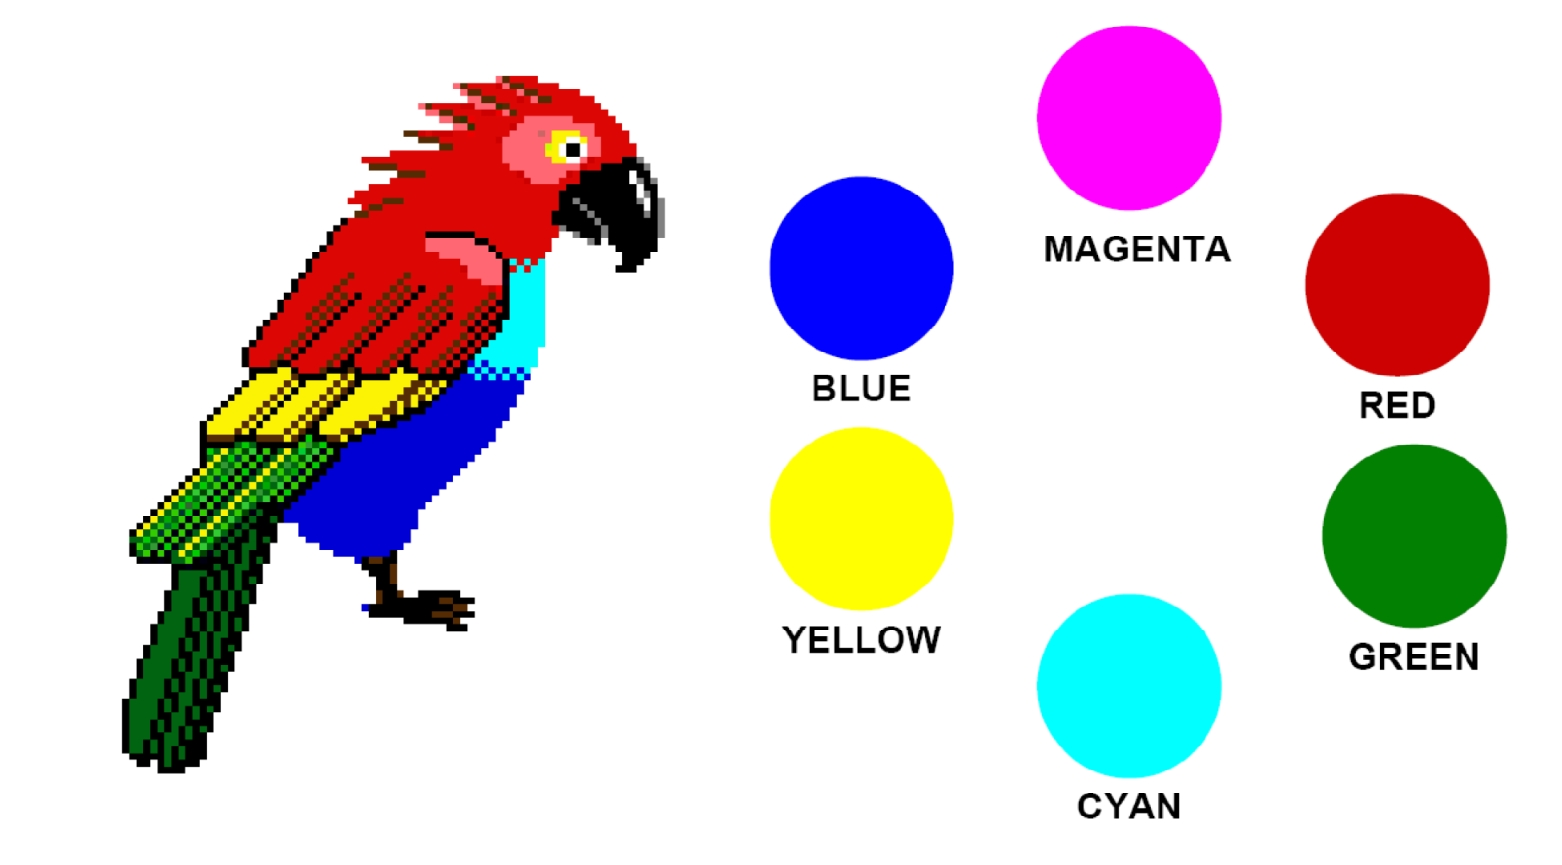
\includegraphics[scale=0.25]{pw}
\caption{Original image of the parrot and the color wheel.}
\label{fig:phasediff}
\end{figure}

\captionsetup[figure]{width=5in}
\begin{figure}[h!]
\centering
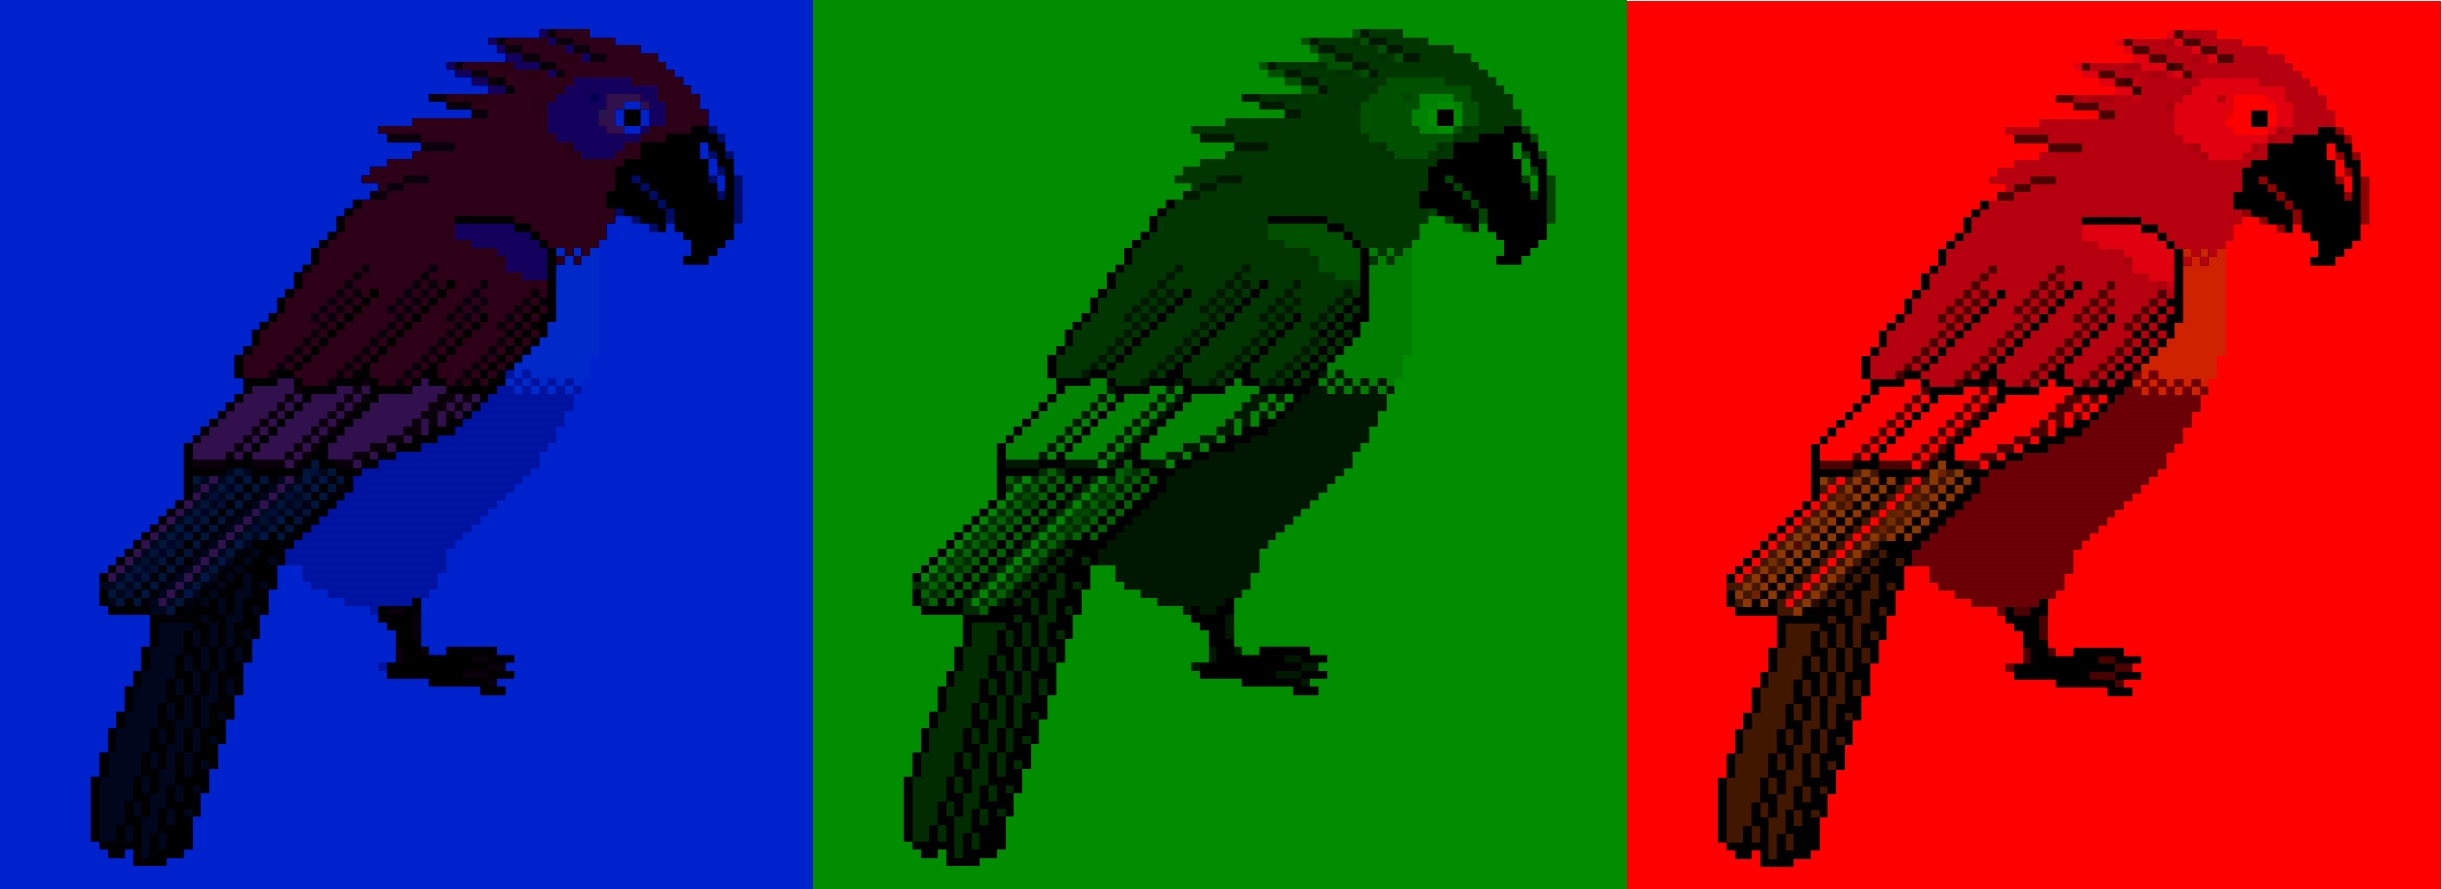
\includegraphics[scale=0.21]{parrot}
\caption{Filtered images for the parrot.}
\label{fig:phasediff}
\end{figure}

\captionsetup[figure]{width=5in}
\begin{figure}[h!]
\centering
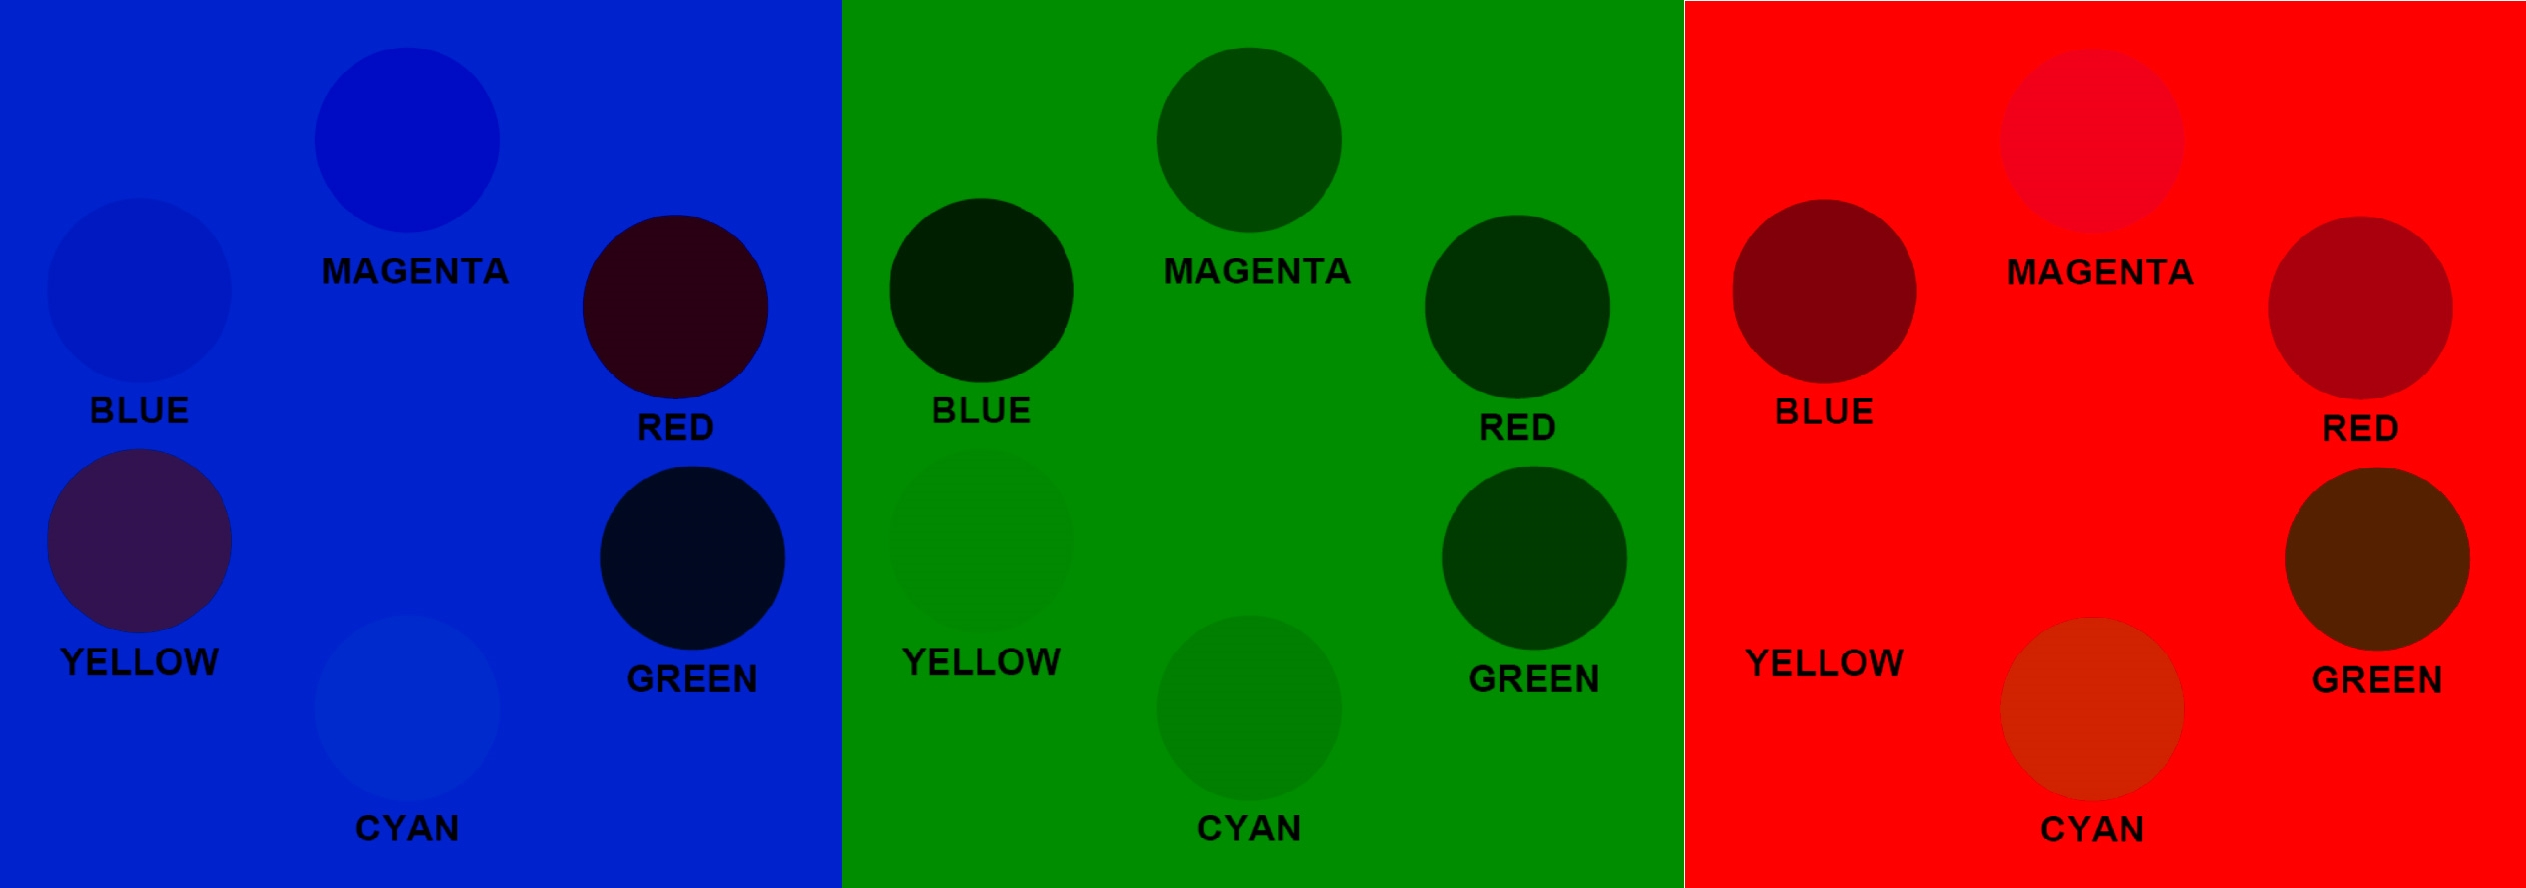
\includegraphics[scale=0.2]{wheel}
\caption{Filtered images for the wheel.}
\label{fig:phasediff}
\end{figure}

\newpage
\section*{Appendix B: Light Ray Box}
\label{sec:appendixA}

\captionsetup[figure]{width=5in}
\begin{figure}[h!]
\centering
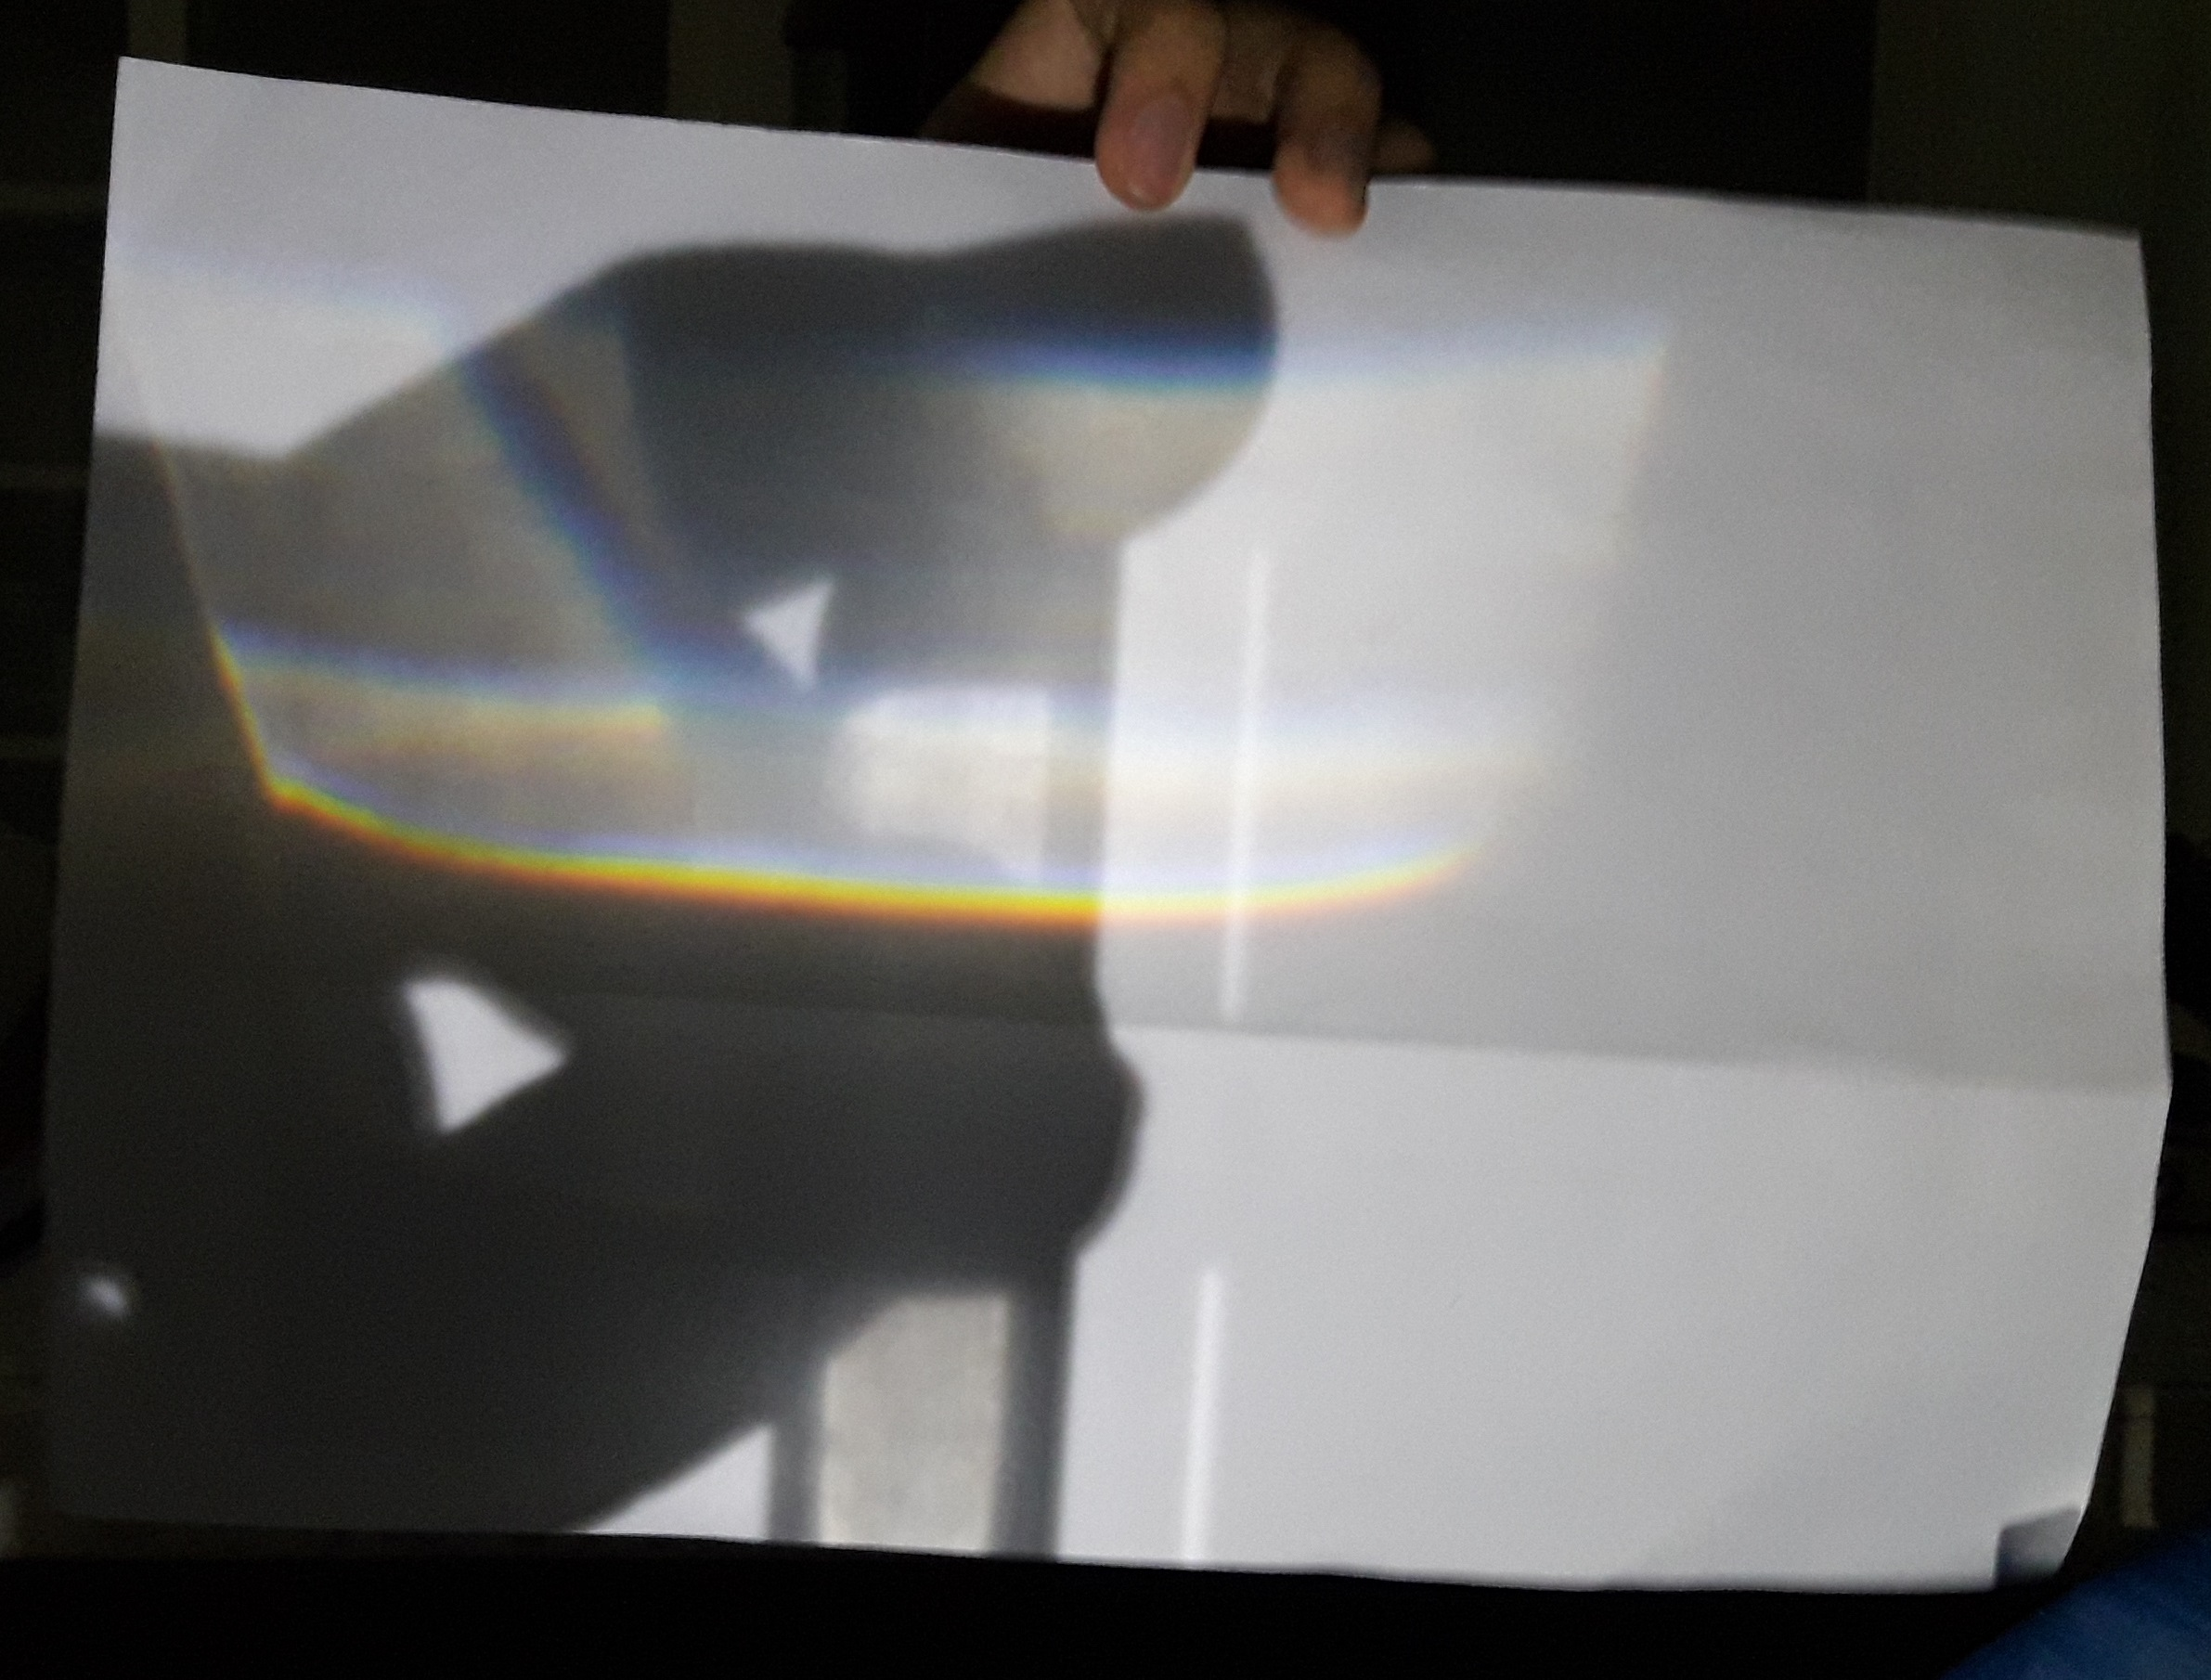
\includegraphics[scale=0.1]{20160922_145952}
\caption{The scattered white light from the light ray box onto the paper.}
\label{fig:phasediff}
\end{figure}

\captionsetup[figure]{width=5in}
\begin{figure}[h!]
\centering
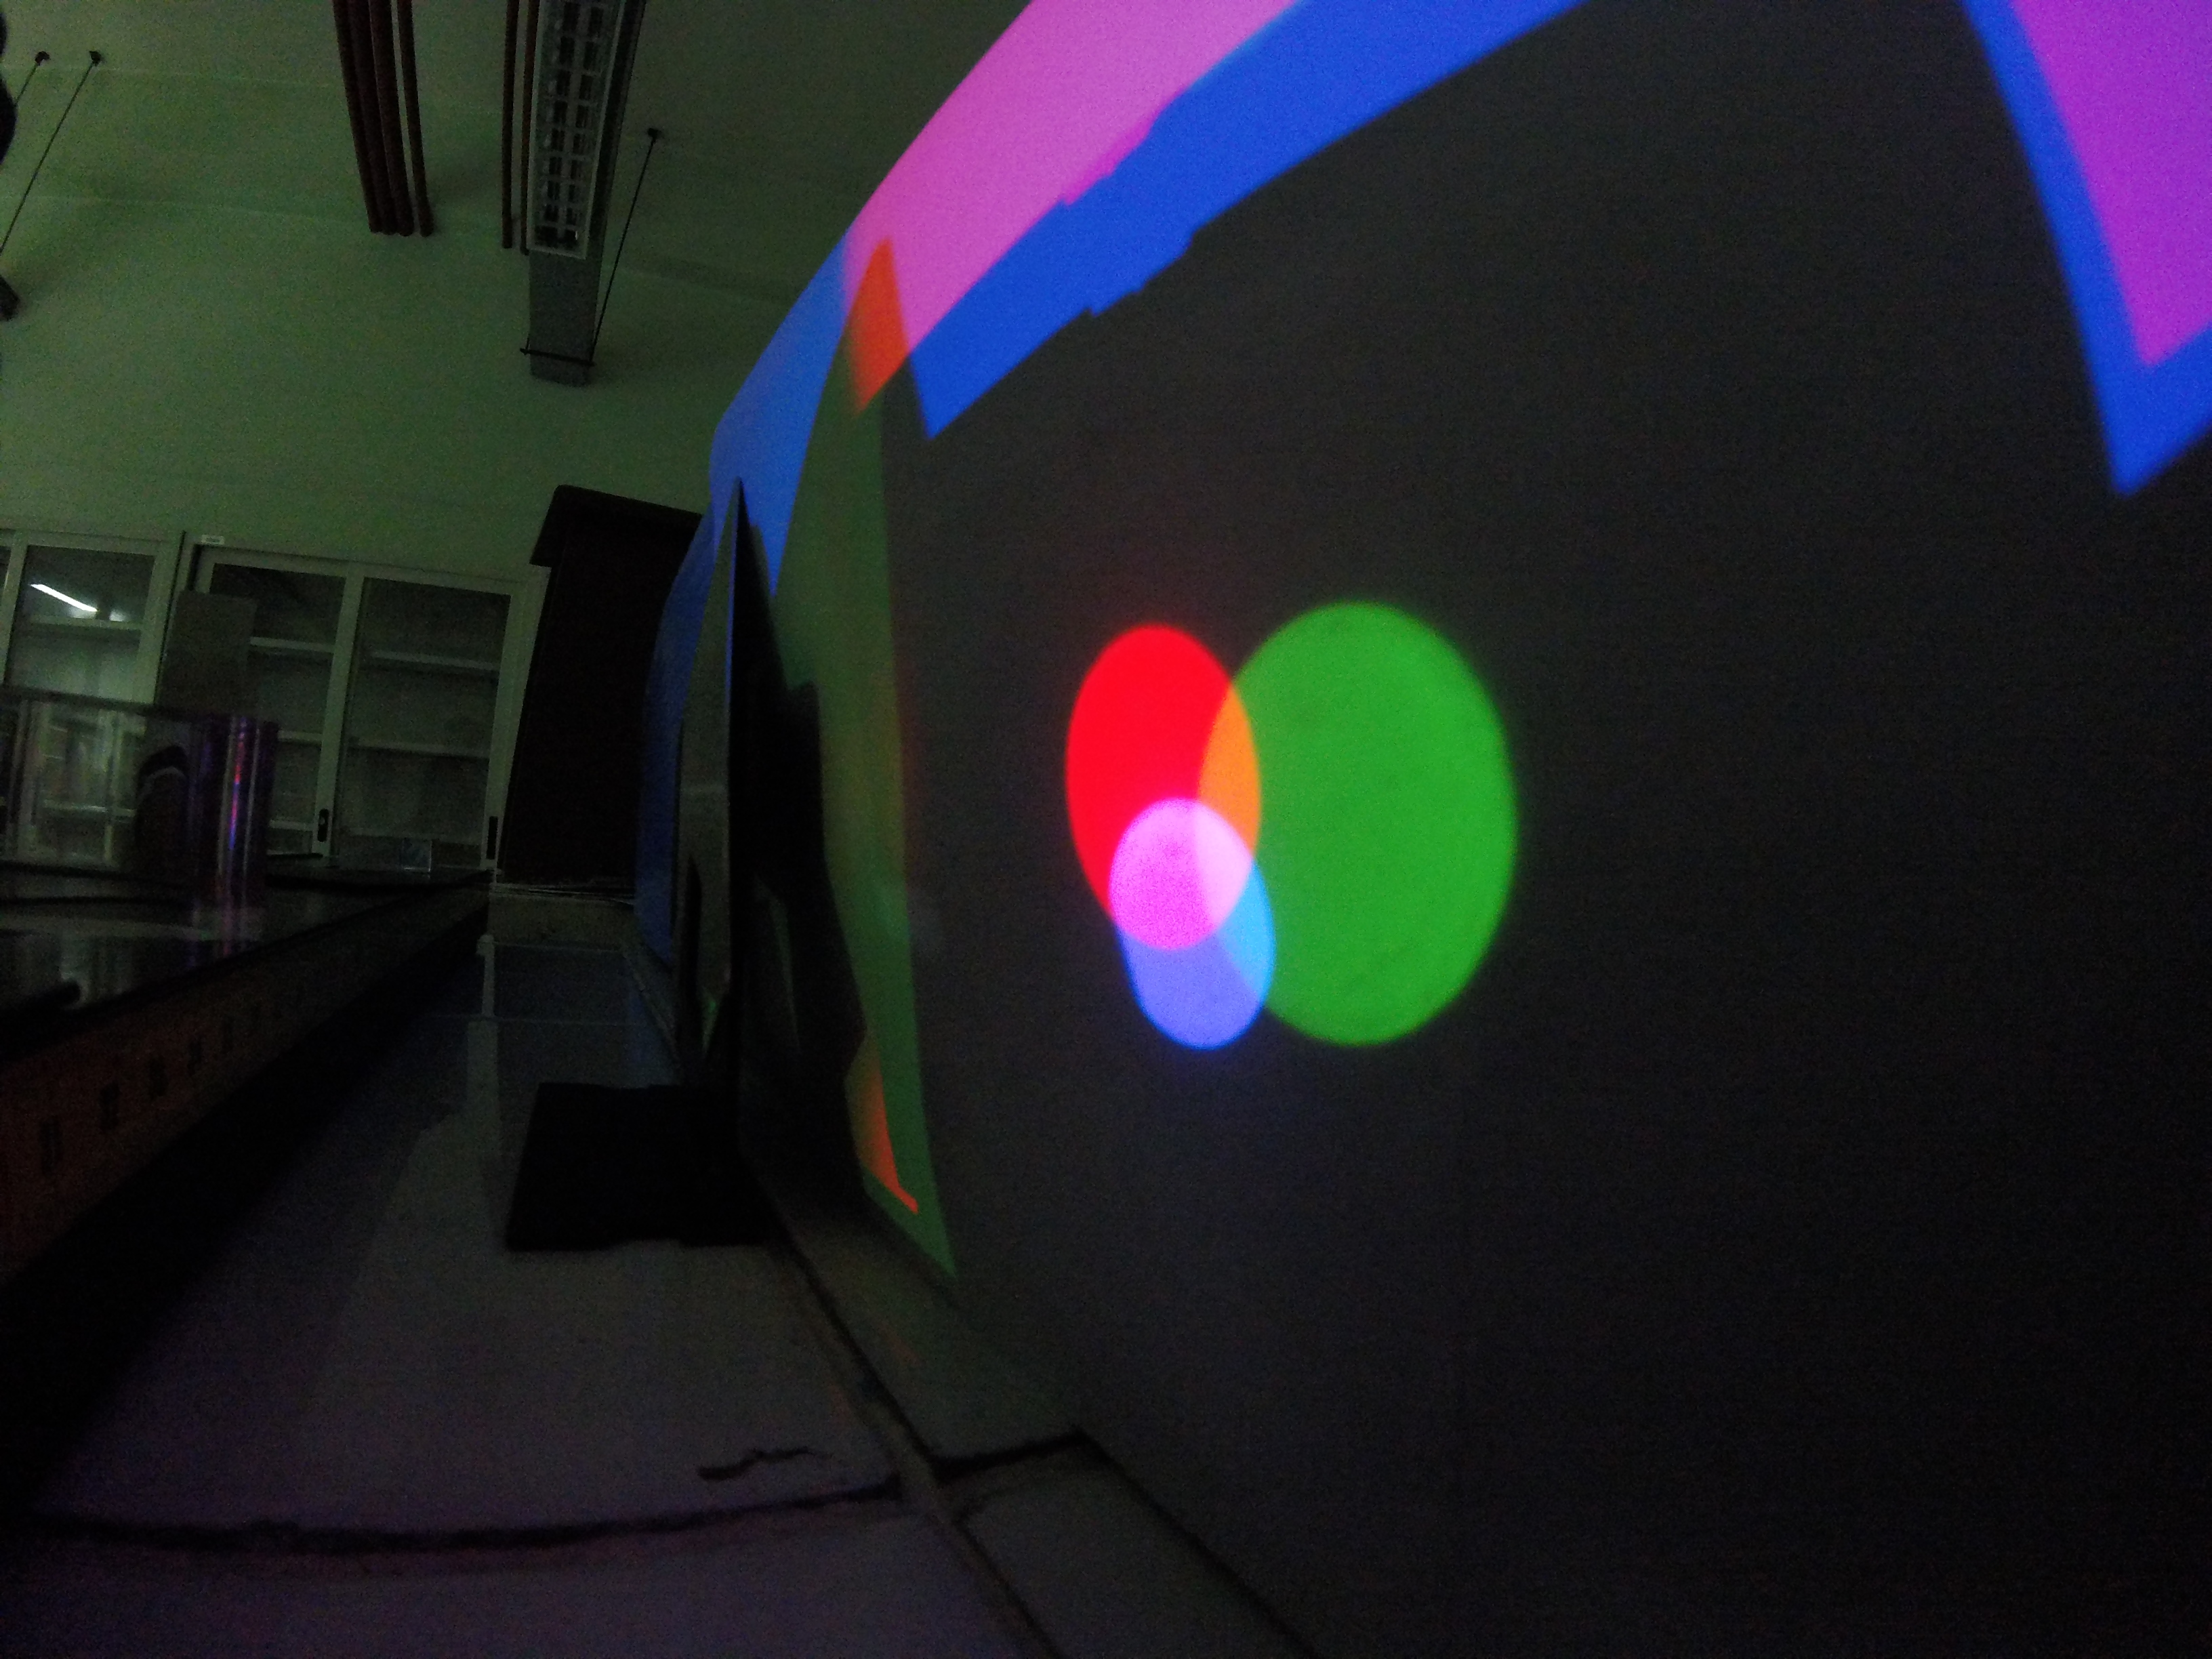
\includegraphics[scale=0.07]{venn}
\caption{The overlapping circles of the primary colors of light.}
\label{fig:phasediff}
\end{figure}


\newpage
\section*{Appendix C: Spotlights}
\label{sec:appendixA}

\captionsetup[figure]{width=5in}
\begin{figure}[h!]
\centering
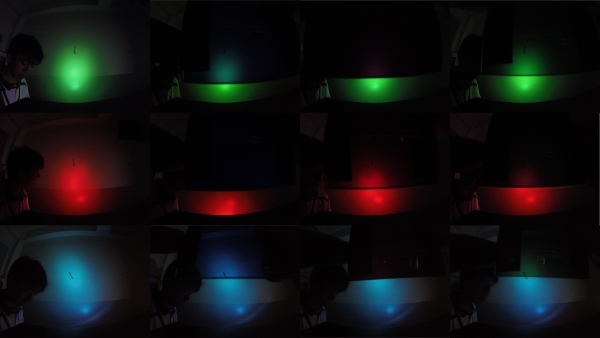
\includegraphics[scale=0.5]{filters}
\caption{Colored spotlights with filters of (from left to right) none, blue, red, and green.}
\label{fig:phasediff}
\end{figure}

\captionsetup[figure]{width=5in}
\begin{figure}[h!]
\centering
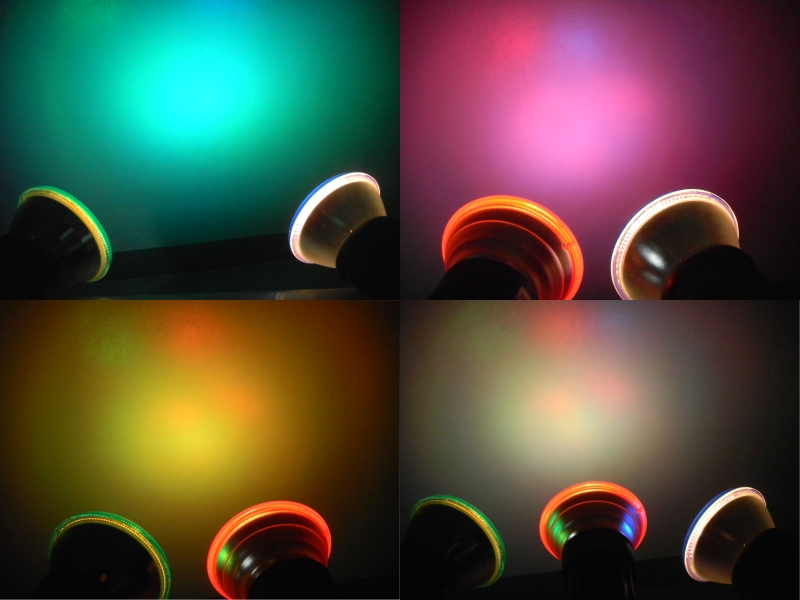
\includegraphics[scale=0.4]{add}
\caption{Overlapping colored spotlights forming (top left) cyan, (top right) magenta, (bottom left) yellow and (bottom right) white.}
\label{fig:phasediff}
\end{figure}

\captionsetup[figure]{width=5in}
\begin{figure}[h!]
\centering
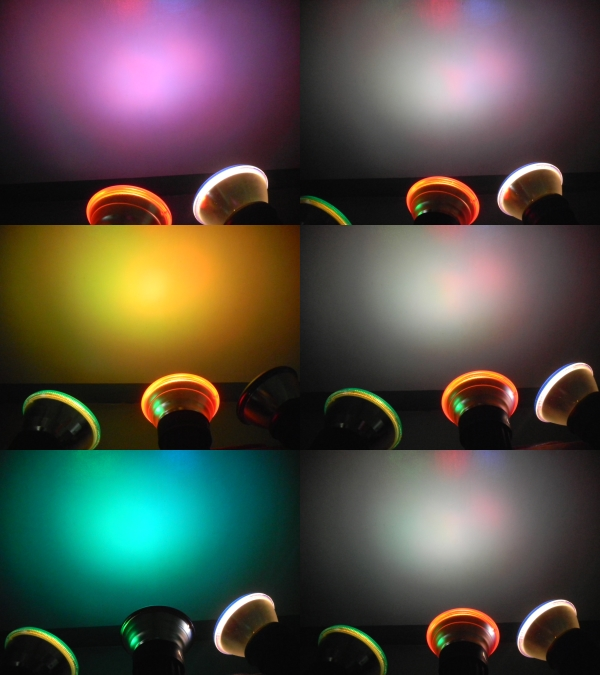
\includegraphics[scale=0.4]{compli}
\caption{Overlapping colored spotlights of (top to bottom) magenta, yellow and cyan. (right) White light achieved from shining (top to bottom) magenta and green, yellow and blue, and cyan and red.}
\label{fig:phasediff}
\end{figure}

\captionsetup[figure]{width=5in}
\begin{figure}[h!]
\centering
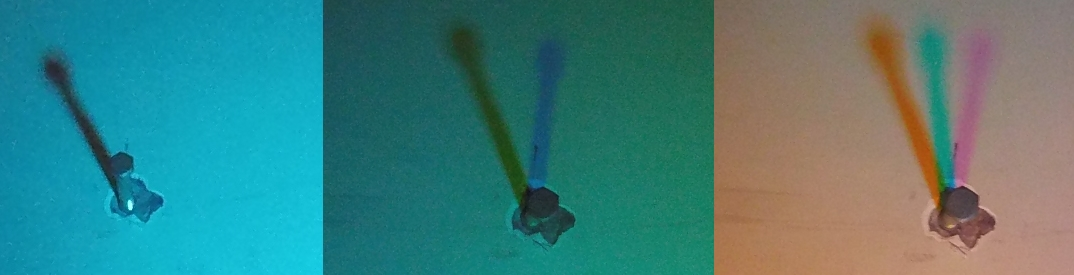
\includegraphics[scale=0.4]{shad}
\caption{Shadows formed from a set-up of green-red-blue spotlights arranged respectively.}
\label{fig:phasediff}
\end{figure}

\captionsetup[figure]{width=5in}
\begin{figure}[h!]
\centering
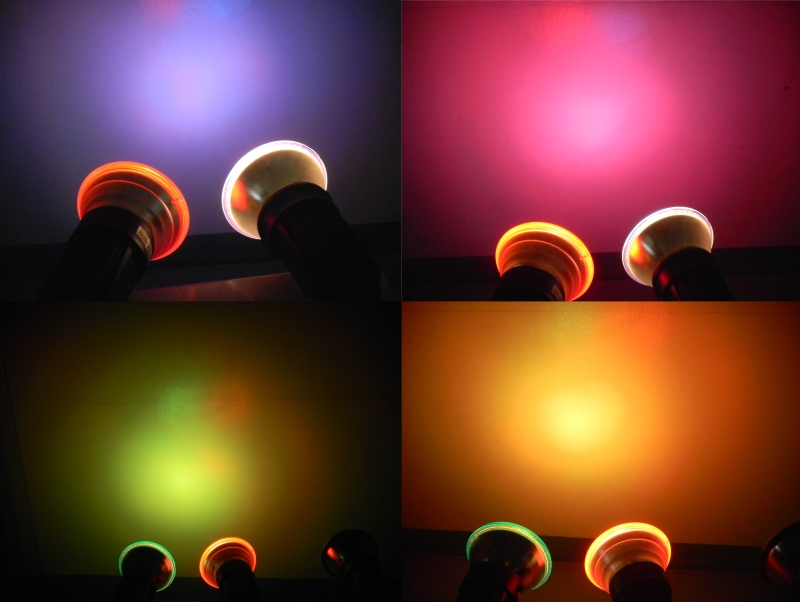
\includegraphics[scale=0.4]{advadd}
\caption{Colors formed after mixing (clockwise from top left) bright blue and dim red, dim blue and bright red, bright red and dim green, and dim red and bright green to form purple, pink, orange and brown, respectively.}
\label{fig:phasediff}
\end{figure}

\end{document}